\documentclass[12pt]{article}
\usepackage[pdftex]{color, graphicx}
\usepackage{amsmath, amsfonts, amssymb, mathrsfs}
\usepackage{dcolumn}
\usepackage{natbib}
\usepackage{wrapfig}
\usepackage{subfig}
\usepackage{float}
\bibpunct{(}{)}{;}{a}{}{,}

\oddsidemargin=0.25in
\evensidemargin=0.25in
\textwidth=6in
\textheight=8.75in
\topmargin=-.5in
\footskip=0.5in


\date{due Sep 10th}

\title{Homework2}



\begin{document}

%\maketitle
\newcommand{\argmin}{\text{argmin}}

\noindent STAT5014\\
 Due Sep.10th

\begin{center}
\noindent
\section*{Homework 2} %this is a comment
\noindent Yin Yuan\\

\vspace{.25 in}
\end{center}
%\begin{enumerate}
 Summary of iris data set
% latex table generated in R 3.0.2 by xtable 1.7-3 package
% Tue Sep  9 22:52:36 2014
\begin{table}[ht]
\centering
\begin{tabular}{rlllll}
  \hline
 &  SepalLength &   SepalWidth &  PetalLength &   PetalWidth \\ 
  \hline
Min.       &4.300   & 2.000   & 1.000   & 0.100    \\ 
1st Qu.    &5.100   & 2.800   & 1.600   & 0.300    \\ 
Median     &5.800   & 3.000   & 4.350   & 1.300    \\ 
Mean       &5.843   & 3.057   & 3.758   & 1.199   \\ 
3rd Qu.    &6.400   & 3.300   & 5.100   & 1.800    \\ 
Max.       &7.900   & 4.400   & 6.900   & 2.500   \\ 
   \hline   
\end{tabular}
\caption{the summary of iris data set}
\end{table}\\

For three species involved in the iris data set, four variables are measured for each of the species, which are sepal length, seppal width, petal length, and petal width.

``Generally'',as shown by the table 1,the minimum value of Sepal length is 4.3,maximum value is 7.9, and mean value is 5.843. As for the sepal width, the minimum is 2.0, maximum is 4.4 and mean is 3.057. Coming to the petal length, the minimum is 1.0, maximum is 6.9, and mean is 3.758. Finally, the petal width's minimum is 0.1, maximum is 2.5 and mean is 1.199. The sepal length and sepal width have a bigger value compared with the petal lenght and petal width respectively.




%\end{enumerate}

\begin{figure*}[hptb]
	\centering
\subfloat[Sepal length by Species]{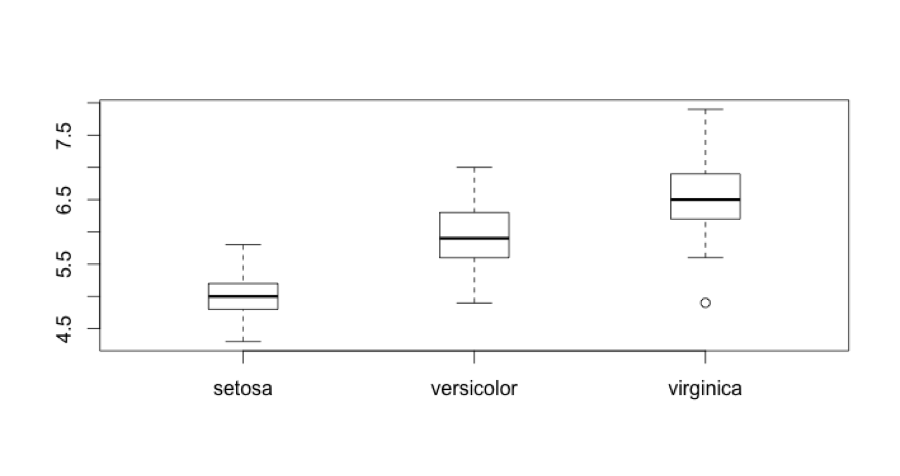
\includegraphics[scale=0.45]{/Users/tonycao/Downloads/hw2/figure1.png}} \;
\subfloat[Sepal width by Species]{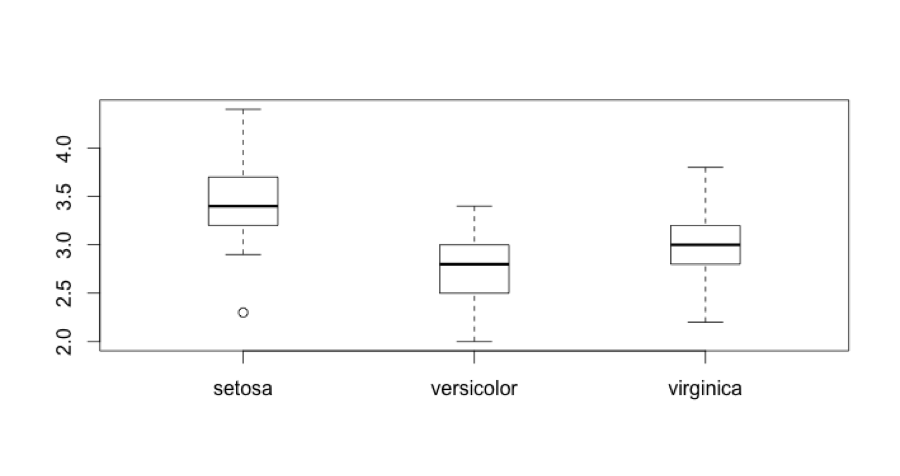
\includegraphics[scale=0.45]{/Users/tonycao/Downloads/hw2/figure2.png}} \\
\subfloat[Petal length by Species]{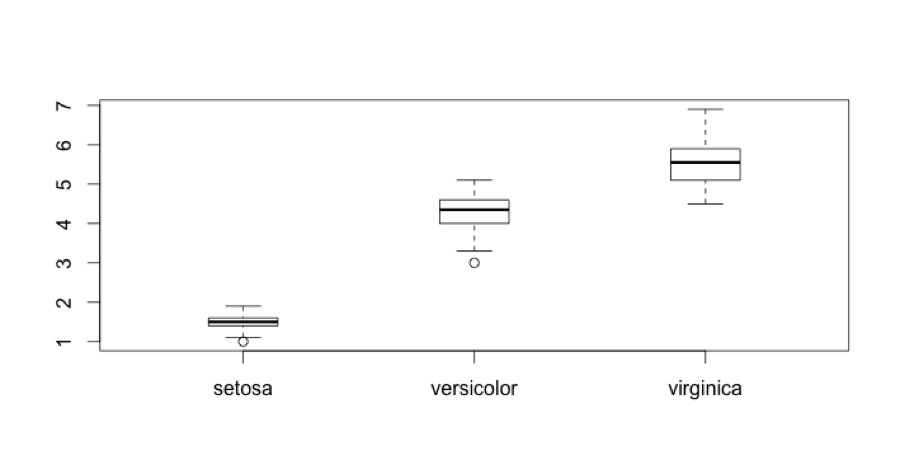
\includegraphics[scale=0.45]{/Users/tonycao/Downloads/hw2/figure3.png}}\;
\subfloat[Petal width by Species]{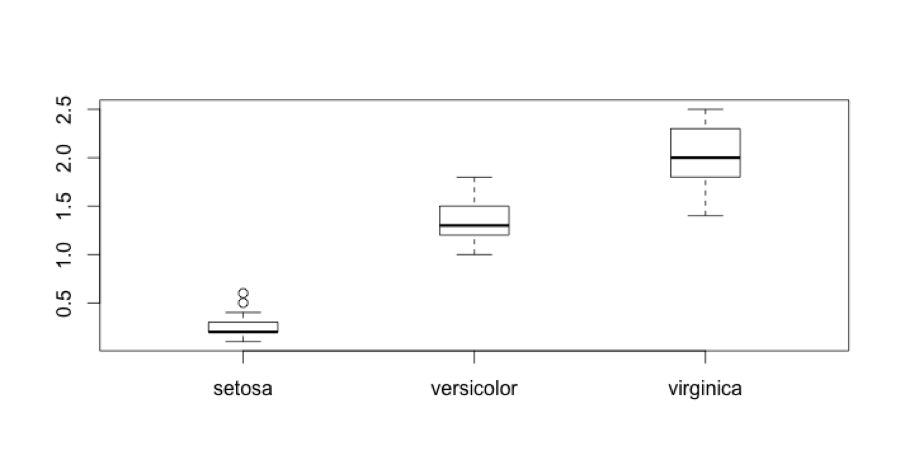
\includegraphics[scale=0.45]{/Users/tonycao/Downloads/hw2/figure4.png}} 
	\caption{title.}
	\label{fig:img}
\end{figure*}

\section*{Add a pdf figure to directory this file is stored in.}
Code for the figure commented out below:

%\begin{figure}[h!]
%  \centering
%  \includegraphics[width=6.5in, keepaspectratio=true]{_.pdf} %replace underscore with name of file.  I recommend converting figures to PDF before using in LaTeX.
%  \caption{Residual plots can be very revealing! \label{fig:resBayes}}
%\end{figure}
%\end{center}
\end{document}



